\subsection{Glyph: \glyph{Unit of information}}
\label{sec:unitInfo}

When representing biological entities, it is often necessary to convey some abstract information about the entity's function that does is not related to its role in the map.  The \glyph{unit of information} is a decoration that can be used in this situation to add information to an EPN.  Some example uses include: characterizing a logical part of an entity such as a functional domain (a binding domain, a catalytic site, a promoter, etc.), or the information encoded in the entity (an exon, an open reading frame, etc.).  A \glyph{unit of information} can also convey information about the physical environment, or the specific type of biological entity it is decorating. A \glyph{unit of information} is represented by a rectangle overlapping the border of the \glyph{EPN} being annotated.

The label carried by \glyph{unit of information} defines the information it carries.  For certain predefined types of information having controlled vocabularies associated with them, SBGN defines specific prefixes that must be included in the label to indicate the type of information in question.  The controlled vocabularies predefined in \SBGNPDLone are described in \sect{CVs}.

\begin{figure}[H]
  \centering
  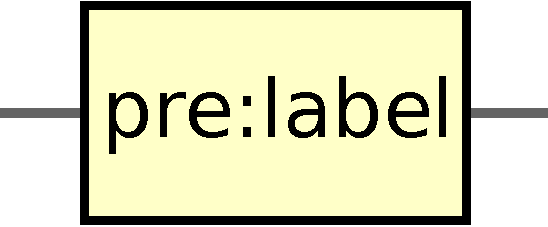
\includegraphics[scale = 0.3]{images/unitInformation}
  \caption{The \PD glyph for \glyph{unit of information}.}
  \label{fig:unitInfo}
\end{figure}




% The following is for [X]Emacs users.   Please leave in place.
% Local Variables:
% TeX-master: "../sbgn_PD-level1"
% End:


